% Copyright (c) 2008-2009 solvethis
% Copyright (c) 2010-2016 Casper Ti. Vector
% Public domain.
%
% 使用前请先仔细阅读 pkuthss 和 biblatex-caspervector 的文档,
% 特别是其中的 FAQ 部分和用红色强调的部分。
% 两者可在终端/命令提示符中用
%   texdoc pkuthss
%   texdoc biblatex-caspervector
% 调出。

% 采用了自定义的(包括大小写不同于原文件的)字体文件名,
% 并改动 ctex.cfg 等配置文件的用户请自行加入 nofonts 选项;
% 其它用户不用加入 nofonts 选项,加入之后反而会产生错误。
\documentclass[UTF8]{pkuthss}

% 使用 biblatex 排版参考文献,并规定其格式(详见 biblatex-caspervector 的文档)。
% 这里按照英文文献在前,中文文献在后排序(“sorting = ecnty”);
% 若需按照中文文献在前,英文文献在后排序,请设置“sorting = centy”;
% 若需按照引用顺序排序,请设置“sorting = none”。
% 若需在排序中实现更复杂的需求,请参考 biblatex-caspervector 的文档。
\usepackage[backend = biber, style = caspervector, utf8, sorting = ecnty]{biblatex}

% 按学校要求设定参考文献列表中的条目之内及之间的距离。
\setlength{\bibitemsep}{3bp}
% 对于 linespread 值的计算过程有兴趣的同学可以参考 pkuthss.cls。
\renewcommand*{\bibfont}{\zihao{5}\linespread{1.27}\selectfont}

% 设定文档的基本信息。
\pkuthssinfo{
	cthesisname = {博士研究生学位论文}, ethesisname = {Doctor Thesis},
	ctitle = {测试文档}, etitle = {Test Document},
	cauthor = {某某},
	eauthor = {Test},
	studentid = {0123456789},
	date = {某年某月},
	school = {某某学院},
	cmajor = {某某专业}, emajor = {Some Major},
	direction = {某某方向},
	cmentor = {某某教授}, ementor = {Prof.\ Somebody},
	ckeywords = {其一,其二}, ekeywords = {First, Second}
}
% 载入参考文献数据库(注意不要省略“.bib”)。
\addbibresource{thesis.bib}

% 普通用户可删除此段,并相应地删除 chap/*.tex 中的
% “\pkuthssffaq % 中文测试文字。”一行。
\usepackage{color}
\def\pkuthssffaq{%
	\emph{\textcolor{red}{pkuthss 文档模版最常见问题:}}

	\texttt{\string\cite}、\texttt{\string\parencite} %
	和 \texttt{\string\supercite} 三个命令分别产生%
	未格式化的、带方括号的和上标且带方括号的引用标记:%
	\cite{test-en},\parencite{test-zh}、\supercite{test-en, test-zh}。

	若要避免章末空白页,请在调用 pkuthss 文档类时加入 \texttt{openany} 选项。

	如果编译时不出参考文献,
	请参考 \texttt{texdoc pkuthss}“问题及其解决”一章
	“其它可能存在的问题”一节中关于 biber 的说明。
}

\begin{document}
	% 以下为正文之前的部分,默认不进行章节编号。
	\frontmatter
	% 此后到下一 \pagestyle 命令之前不排版页眉或页脚。
	\pagestyle{empty}
	% 自动生成封面。
	\maketitle
	% 版权声明。封面要求单面打印,故需新开右页。
	\cleardoublepage
	% Copyright (c) 2008-2009 solvethis
% Copyright (c) 2010-2017 Casper Ti. Vector
% All rights reserved.
%
% Redistribution and use in source and binary forms, with or without
% modification, are permitted provided that the following conditions are
% met:
%
% * Redistributions of source code must retain the above copyright notice,
%   this list of conditions and the following disclaimer.
% * Redistributions in binary form must reproduce the above copyright
%   notice, this list of conditions and the following disclaimer in the
%   documentation and/or other materials provided with the distribution.
% * Neither the name of Peking University nor the names of its contributors
%   may be used to endorse or promote products derived from this software
%   without specific prior written permission.
%
% THIS SOFTWARE IS PROVIDED BY THE COPYRIGHT HOLDERS AND CONTRIBUTORS "AS
% IS" AND ANY EXPRESS OR IMPLIED WARRANTIES, INCLUDING, BUT NOT LIMITED TO,
% THE IMPLIED WARRANTIES OF MERCHANTABILITY AND FITNESS FOR A PARTICULAR
% PURPOSE ARE DISCLAIMED. IN NO EVENT SHALL THE COPYRIGHT HOLDER OR
% CONTRIBUTORS BE LIABLE FOR ANY DIRECT, INDIRECT, INCIDENTAL, SPECIAL,
% EXEMPLARY, OR CONSEQUENTIAL DAMAGES (INCLUDING, BUT NOT LIMITED TO,
% PROCUREMENT OF SUBSTITUTE GOODS OR SERVICES; LOSS OF USE, DATA, OR
% PROFITS; OR BUSINESS INTERRUPTION) HOWEVER CAUSED AND ON ANY THEORY OF
% LIABILITY, WHETHER IN CONTRACT, STRICT LIABILITY, OR TORT (INCLUDING
% NEGLIGENCE OR OTHERWISE) ARISING IN ANY WAY OUT OF THE USE OF THIS
% SOFTWARE, EVEN IF ADVISED OF THE POSSIBILITY OF SUCH DAMAGE.

% 此处不用 \specialchap,因为学校要求目录不包括其自己及其之前的内容。
\chapter*{版权声明}
% 综合学校的书面要求及 Word 模版来看,版权声明页不需加页眉、页脚。
\thispagestyle{empty}

任何收存和保管本论文各种版本的单位和个人,
未经本论文作者同意,不得将本论文转借他人,
亦不得随意复制、抄录、拍照或以任何方式传播。
否则一旦引起有碍作者著作权之问题,将可能承担法律责任。

% 若需排版二维码,请将二维码图片重命名为“barcode”,
% 转为合适的图片格式,并放在当前目录下,然后去掉下面 2 行的注释。
\vfill\noindent

\includegraphics[height = 5em]{barcode}

% vim:ts=4:sw=4


	% 此后到下一 \pagestyle 命令之前正常排版页眉和页脚。
	\cleardoublepage
	\pagestyle{plain}
	% 重置页码计数器,用大写罗马数字排版此部分页码。
	\setcounter{page}{0}
	\pagenumbering{Roman}
	% 中英文摘要。
	\begin{cabstract}
随着互联网的快速发展,以用户产生内容为标志的Web2.0时代到来,大量且庞杂的信息充斥着人们的日常生活。
推荐系统可以对海量信息进行筛选、过滤,将用户最关注最感兴趣的信息展现在用户面前,能大大增加这些内容的转化率,
对各类应用系统都有非常巨大的价值,逐渐成为互联网平台中不可或缺的一环。
大数据时代的来临积累了大量的用户数据,同时计算机硬件性能的大幅度提升,这些改变带了深度学习的风靡兴起。
深度学习作为一种机器学习范式,利用定制的神经网络结构对学习任务进行建模,
直接从原始数据向预测目标进行端到端的转换,省去了大量的构建特征工程的人工花销。
深度学习在语音识别、图像识别等诸多研究领域上取得了突破性的进展,将人工智能引上了一个新的台阶。

鉴于深度学习在诸多研究领域的成功应用和突破性进展,近些年来,如何将深度学习成功应用于推荐系统领域中成为了研究者们的热门话题。
在本文中,我们提出了多层感知器模型和长短期兴趣模型尝试使用深度学习来解决推荐系统中的电影评分预测任务。
首先,我们将电影评分预测任务看成一个回归问题,
基于神经网络中经典的多层感知器提出了UM模型(User Movie Model)和U-M模型(User minus Movie Model),
利用嵌入技术将用户和电影信息压缩至低维的向量表示,并且输入到多层感知器中的输入层中,通过隐藏层的学习和映射,在输出层输出预测评分数据。
UM模型和U-M模型是使用神经网络对求解推荐问题进行的初步探索,取得了和经典推荐算法相近的实验效果,展示了深度学习在推荐系统中应用的可行性。

其次,针对用户兴趣随时间流逝发生漂移的特点,我们提出了长短期兴趣模型LSIM(Long Short Interest Model),
将用户的兴趣分成长期兴趣和短期兴趣两种,并且认为位于相同短期兴趣中的物品(本文场景中是电影)之间具有更高的相似度。
利用观看过的电影生成对应的用户刻画长期兴趣,利用用户和同一个时间窗口内的邻居电影生成对应的电影刻画短期兴趣,
得到带有时序特征的用户表示和电影表示。最后使用基于特征的矩阵分解算法融合用户表示和电影表示,生成所有的待预测评分。
在两类真实世界数据集上进行的大量实验表明了长短期兴趣模型在预测准确率上都超过经典的协同过滤算法,
同时和目前最优模型的结果十分接近,证明了长短期兴趣模型的算法有效性。

除了理论实验部分,本文还实现了一个电影推荐原型系统MovieRec。MovieRec从多个来源(如MovieLens,IMDb,TMDb等网站)获取电影的详细属性,
帮助用户更好地了解一部电影的各个方面。同时还根据用户的历史评分数据,实现了本文提出的多层感知器模型和长短期兴趣模型,
以及经典的矩阵分解算法和因式分解机算法,用户可以根据自己的爱好进行切换和选择。最后对于推荐结果,MovieRec还提供了显式的反馈接口,
用户可以通过点赞或者差评的方式反映对推荐结果的满意程度,系统会根据用户的反馈进行推荐结果的动态调整。
\end{cabstract}

\begin{eabstract}
With the rapid development of the Internet, the Web2.0 era comes, as a result,
a great deal of user-generated information floods people's daily life.
Recommender system can filter the massive information, 
find the most concerned and interesting information to display in front of users,
which could greatly increase the conversion rate of these content.
Meanwhile, recommender system is valuable for vast types of applications,
and gradually becomes an indispensable part of most Internet platforms.
Big data era has accumulated lots of data, while the computer hardware performance has won a huge upgrade,
these changes make deep learning spring up rapidly. Deep learning, as a machine learning paradigm,
takes advantage of custom neural network structures to model the learning task,
performs directly end-to-end conversions from the raw data to the forecasting target,
with the goal to save the cost of artificial feature engineering.
Deep learning has made breakthrough improvement in many research fields,
such as speech recognition and image recognition, help lead artificial intelligence to a new level.

In view of these successful applications and breakthrough developments of deep learning in many research fields,
it has become a hot topic for researchers to successfully apply deep learning to recommender system in recent years.
In this paper, we propose multilayer perceptron model and long-short interest model,
which aims to use deep learning to solve the movie rating prediction task in recommender system.
Firstly, we consider the movie rating prediction task as a regression problem.
Based on the classic multi-layer perceptron in neural network,
we propose UM model (User Movie Model) and U-M model (User minus Movie Model).
The user and movie information are compressed into a low-dimensional vector representation using the embedding technique,
then they are inputted into a multi-layer perceptron, the predicted ratings are outputted after hiding layer learning.
UM model and U-M model are the initial explorations to use neural network to solve the recommender problems,
and the experimental results are similar to the classical recommender algorithms,
which shows the feasibility of the application of deep learning in recommender system.

Secondly, we take the characteristics that user interest drifts over time into account, propose the long short interest model.
The user's interest is divided into two kinds: long-term interest and short-term interest,
and there is a higher similarity between the movies located in the same short-term interest.
Long-term interest is expressed via using all the watched movies to generate the corresponding user,
while short-term interest is expressed via using the user and the neighbor movies
in the same time window to generate the corresponding movie.
The user representation and movie representation, which contains sequential characteristics,
can be obtained after the generation process.
Finally, the feature-based matrix factorization algorithm is used to merge user representation and movie representation,
to generate all the predicted ratings.
A large number of experimental results show that the long-short interest model reveals a great improvement
than traditional collaborative filtering algorithms in the prediction accuracy.
Meanwhile our results are very close to the state-of-the-art ones,
which shows the effectiveness of the long-short interest model.

In addition to the theoretical and experimental part, this paper also implements a movie recommendation prototype system MovieRec. MovieRec obtains the detailed properties of a movie from a number of sources (such as MovieLens, IMDb, TMDb and other sites),
to help users better understand all aspects of the movie.
At the same time, MovieRec realizes our proposed multilayer perceptron model and long-short interest model,
and classic matrix factorization algorithm and factorization machine algorithm,
to recommend movie to users according to the users' historical ratings data.
Finally, for the recommended results, MovieRec also provides a feedback interface,
users could tell the system whether the recommended results are good or bad,
the system will dynamic adjust the recommend results based on users' feedbacks.
\end{eabstract}



	% 自动生成目录。
	\tableofcontents

	% 以下为正文部分,默认要进行章节编号。
	\mainmatter
	% 序言。
	% Copyright (c) 2014,2016 Casper Ti. Vector
% Public domain.

\specialchap{序言}
\pkuthssffaq % 中文测试文字。

% vim:ts=4:sw=4

	% 各章节。
	\chapter{绪论}
\section{推荐系统的研究背景}
近些年,随着信息科技的广泛应用和迅猛发展,互联网正在渗透我们日常生活中的各个方面,人们逐渐从信息匮乏的时代
走入了信息过载(Information Overload)的时代。为了解决信息过载的问题,诸多富有创造力的解决方案被提出,
其中最具代表性的是分类目录,搜索引擎和推荐系统(Recommender System)。采用分类目录方案的代表包括国外的雅虎
\footnote{https://www.yahoo.com}和国内的Hao123\footnote{https://www.hao123.com},
它们的核心功能是将流行的网站分门别类,为用户提供免费的网站导航,将用户引导至感兴趣的网站上。
但随着互联网规模的不断扩大,分类目录网站覆盖的少量热门网站也越来越难以满足用户的需求,搜索引擎技术应运而生。
著名的搜索引擎网站包括国外的谷歌\footnote{https://www.google.com}和国内的百度\footnote{https://www.baidu.com},
通过这些网站,用户只需要输入几个关键词就可以获取高度相关的信息。和搜索引擎一样,推荐系统也是一种帮助人们
快速寻找感兴趣信息的解决方案,不同的是,推荐系统不需要用户提供明确的信息需求,而是通过用户的历史行为进行兴趣建模,
从而提供满足用户兴趣的信息。可以说搜索引擎和推荐系统相辅相成,一个满足了用户有明确信息需求时的信息检索,
另一个满足了用户没有明确信息需求时的信息推荐。

\begin{figure}[htbp]
\centering

\includegraphics[scale=0.26]{images/taobao.jpeg}
\caption{淘宝网上的商品推荐样例}
\label{fig:taobao}
\end{figure}

千禧年伊始,互联网逐渐从以编辑为主体的Web1.0时代进入以用户为主体的Web2.0时代,大量用户生成数据充斥着网络,
信息爆炸式地增长,标志着大数据时代的到来。电商平台里的商品、媒体网站里的新闻、小说网站里的作品、招聘网站里的职位等,
当数量超过用户可以遍历的上限时,用户开始无法快速获取满足他们需求的信息。推荐系统可以对海量信息进行筛选过滤,
将用户最关注最感兴趣的信息展现在用户面前,能大大增加这些内容的转化率,对各类应用系统都有非常巨大的价值,
逐渐成为互联网平台不可或缺的一环。图\ref{fig:taobao}给出了著名电子商务网站淘宝网上的商品推荐样例。

一般认为,推荐系统成为一个相对独立的研究方向始于1994年美国明尼苏达大学GroupLens研究组推出GroupLens系统
\parencite{resnick1994grouplens},该系统主要有两大重要贡献,一是为推荐问题创建了一个形式化的数学模型,
二是首次提出了基于协同过滤方法完成推荐任务的思想。该系统提出的模型属于一种基于用户的协同过滤算法,之后的几十年,
其他一些协同过滤的算法也相继被提出,其中最具代表性的是基于物品的协同过滤算法\parencite{sarwar2001item}
和基于矩阵分解的协同过滤算法\parencite{koren2009matrix}。
2006年著名的互联网公司Netflix举办的百万美金大奖赛\parencite{bennett2007netflix}可以看做是推荐系统的一次热潮。
全球四万多个团队参赛,经过近三年的较量,获奖队伍终于达到了比赛的设定条件。其使用的方法的核心模块就是矩阵分解,
这使得基于矩阵分解的协同过滤在近十年中得到了学术界和工业界的广泛关注和重视。同时,其他推荐算法也在不断发展,
比如基于内容的推荐\parencite{ricci2011introduction,pazzani2007content},
基于知识库的推荐\parencite{trewin2000knowledge},
以及借助情感分析\parencite{ganu2009beyond}和主题模型\parencite{wang2011collaborative}的基于文本的推荐等等。
另外,这些方法之间的互补与融合也成为了重要的研究方向\parencite{burke2002hybrid}。

\section{深度学习的研究背景}
深度学习(Deep Learning)起源于人工神经网络的研究,是今年来兴起的机器学习范式,
拥有多个隐层的多层感知器(Multi-Layer Perceptron)就是一种深度学习模型。
深度学习利用其多层神经网络结构,通过底层基础特征学习抽象的高层表示特征,
直接尝试解决抽象认知的难题,在语音识别、图像识别和自然语言处理等研究领域取得了突破性的进展。

反向传播算法作为人工神经网络最初的训练算法,由于训练过程中存在梯度消失或梯度爆炸的问题,
以及容易陷入局部最优值的不足,被人们所遗弃。
2006年,Hinton等人\parencite{hinton2006fast}提出深度置信网络(Deep Belief Nets),
通过逐层预训练的方法,为神经网络提供一个较优的初始值,然后进行微调完成训练过程,
从而解决了反向传播算法带来的优化难题。

Lecun等人\parencite{lecun1989backpropagation}提出卷积神经网络
(Convolutional Neural Network, CNN),利用空间相对关系减少参数数目以提高训练性能,
并将其成功应用于图像处理领域,在手写字体识别、图像分割和物体检测等研究领域取得了突破性的进展。
如图\ref{fig:taobao}所示,围棋项目上,AlphaGo\parencite{silver2016mastering}结合卷积神经网络和蒙特卡洛树搜索,
成功击败人类著名棋手李世石,引爆了深度学习的热潮,将人工智能带上了一个新的台阶。深度学习不仅学术意义巨大,
而且实用性很强,工业界也开始了大规模的投入,大量新型产品从中获益。
例如著名电动汽车公司特斯拉推出自动驾驶汽车\parencite{bengio2009learning},在一定程度上能减轻驾驶人员负担,
不仅可帮助减少车祸,还能大幅降低交通拥堵情况。

\begin{figure}[htbp]
\centering
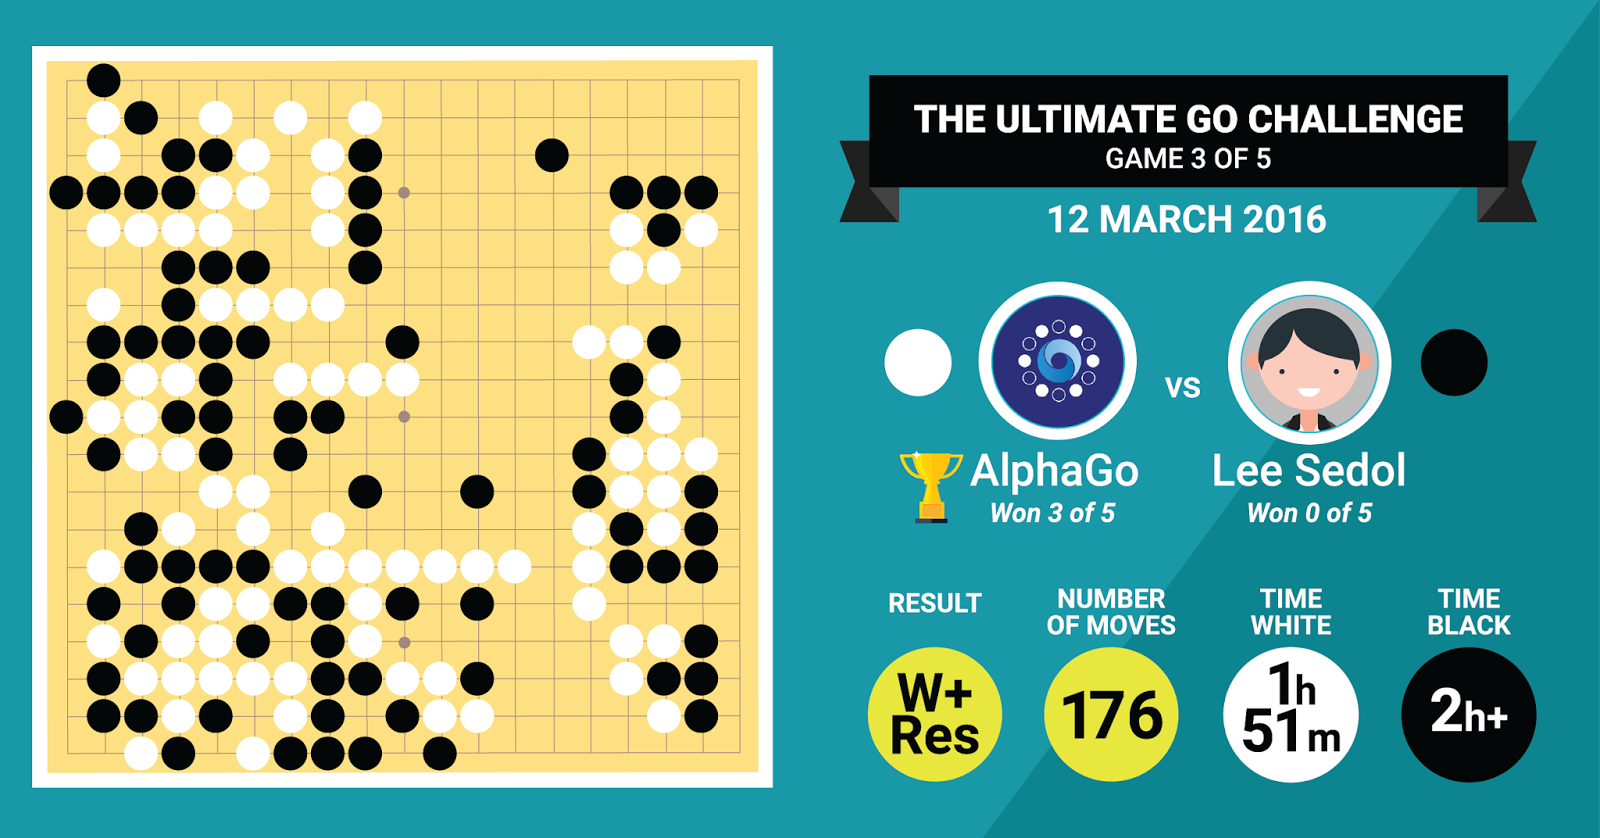
\includegraphics[scale=0.22]{images/alphago.png}
\caption{AlphaGo战胜人类棋手李世石}
\label{fig:alphago}
\end{figure}

自然语言处理与深度学习的初次结合来源于2013年
Mikolov等人\parencite{mikolov2013efficient,le2014distributed,bojanowski2016enriching}提出的Word2Vec模型,
从提出至今,Word2Vec已经成为了深度学习在自然语言处理中的基础部件,
不胜枚举的深度学习模型在表示单词、短语、句子、段落等文本要素时都需要用Word2Vec来做单词级别的向量化。
此后深度学习在自然语言处理领域大显神威,在情感分析\parencite{socher2013recursive}、
问答系统\parencite{li2016deep}、机器翻译\parencite{bahdanau2014neural}等问题上,
以惊人的效果提升,颠覆了使用多年的老方法。
更重要的是,它引起了对主流方法的反思,提供了一个全新的思考视角。

深度学习在推荐系统的应用并不常见,最初的工作来源于2007年Salakhutdinov等人\parencite{salakhutdinov2007restricted}
利用受限莫尔兹曼机(Restricted Boltzmann Machine, RBM)解决Netflix百万美金大奖赛中的电影评分预测任务,
但是之后只有少数几个工作\parencite{phung2009ordinal}继续了该项研究。
当深度学习在图像识别和语音识别领域中取得突破性进展时,开始逐渐有部分工作将深度学习应用于推荐系统中。
Sedhain等人\parencite{sedhain2015autorec}使用自动编码机(AutoEncoder)通过重构评分数据的方式直接进行评分预测,
在多个数据集上取得优异的成绩,但是规避了冷启动的问题,直接使用一个预定义的评分代替那些不能预测的冷启动评分。
Strub等人\parencite{strub2016hybrid}在此基础上进行了改进,使用层叠去燥自动编码机将辅助信息引入进自动编码机学习框架中,
减缓了冷启动造成的负面影响。
Wang等人在\parencite{wang2015collaborative}和\parencite{wang2016collaborative}分别提出
贝叶斯版本的自动编码机和循环神经网络(Recurrent Neural Networks, RNN)来对文本信息进行提取,
融合进概率矩阵分解(Probabilistic Matrix Factorization, PMF)\parencite{salakhutdinov2007probabilistic}的框架中,
在论文推荐场景中取得良好的表现。
2013年Oord等人\parencite{van2013deep},2014年Wang等人\parencite{wang2014improving}
将卷积神经网络引入推荐系统中,从音乐内容的角度出发,解决音乐推荐问题。

\section{本文研究意义}
推荐系统是一个具有很强现实价值的研究领域,优秀的推荐系统不仅可以帮助用户快速获取到感兴趣的物品,
还可以提高物品提供商的转化效率。在当前流行的各类大型网站平台上,
一般都提供了推荐系统的功能方便用户获取自己感兴趣的信息,比如淘宝网站上的商品推荐,或者豆瓣电台中的音乐推荐等。

深度学习是近年来兴起的机器学习范式,通过特定的神经网络结构,直接从原始数据向预测目标进行端到端的转换,
省去了大量的构建特征工程的人力花销,在语音识别、图像识别等诸多研究领域上取得了突破性的进展。

本文正是深度学习应用于推荐系统领域的一次尝试,通过多层感知器模型和长短期兴趣模型解决了电影评分预测任务,
为推荐算法提供了一个新的解题角度。多层感知器模型是一个通用的回归框架,将原始的用户表示和电影表示直接作为输入,
通过多层的神经网络结构一层层地抽象归纳用户和电影的关系,最终得到待预测评分数据。
与此同时,如果真实的推荐环境中还包含各类辅助信息,也可以不进行处理直接加入到多层感知器模型中。

长短期兴趣模型是对传统协同过滤算法的一种扩展。传统的协同过滤算法将同一个用户的交互数据等同视之,这样假设往往是存在问题的。
例如在电商平台上的推荐系统中,采用协同过滤算法时,我们会认为一个用户购买过的商品具有类似的兴趣分布,但实际上随着时间的推移,
用户购买的商品在不同的时间区间往往具有很大的区别。长短期兴趣模型正是用来刻画用户兴趣随时间漂移的现象的一种模型,
在利用评分数据的同时,额外引入了评分时间的信息,让刻画用户兴趣漂移成为了可能,深度学习的框架也保证了可以学习出较好的用户表示和物品表示。
一方面这些较好的用户表示和物品表示可以用在评分预测任务上,另一方面,这些表示还可以帮助发现相似用户和相似电影,
或者异常用户和异常电影,并进行相应的好友推荐或者异常检测等等。

\section{本文主要工作及成果}
本文是深度学习在推荐系统领域应用的一种尝试,提出了多层感知器模型和长短期兴趣模型解决电影评分预测任务,
同时实现了电影推荐原型系统MovieRec用以展示直观的推荐效果。主要包含以下几点成果:

\begin{itemize}
\item
本文利用经典的神经网络结构实现了多层感知器模型,取得了和传统推荐算法相近的实验结果,证明了深度学习应用于推荐系统领域的可行性。
\item
本文针对用户的兴趣分布会随时间流逝发生变化的特点,提出长短期兴趣模型,
在学习过程中融入了时间因素,使得用户模型和物品模型更加具有时效性,从而进一步提升推荐系统的推荐性能。
\item
本文实现了一个电影推荐原型系统MovieRec,将我们提出的多层感知器模型和长短期兴趣模型进行了应用,
可以帮助用户快速发现其可能感兴趣的电影。
\item
本文提出的长短期兴趣模型已经投稿并发表在了第五届自然语言处理与中文计算会议上(NLPCC 2016)。
\end{itemize}

\section{本文篇章结构}
本文一共由六个章节组成。

第一章节是绪论部分,主要介绍了推荐系统和深度学习的研究背景,阐述了本文的研究意义,
然后介绍了我们的主要工作和研究成果,最后描述了本文的篇章结构。

第二章节阐述了推荐系统和深度学习的相关工作,主要包括多种推荐算法的简介,推荐系统的评价方法,
神经网络版本词向量模型,深度学习在推荐系统中的应用实例等相关方法。

第三章节描述了本文提出的基于深度学习的推荐系统算法,主要包含多层感知器模型和长短期兴趣模型。
对于前者,主要介绍了UM模型和U-M模型的算法框架,同时引入了Dropout技术提升算法鲁棒性;
对于后者,主要阐述了如何利用长期兴趣和短期兴趣生成带时序特征的用户表示和电影表示,
并且利用基于特征的矩阵分解框架融合两种表示,最终得到待预测评分的过程。

第四章节展示了本文提出的多层感知器模型和长短期兴趣模型在两类真实世界数据集上的实验效果,
对实验设置、评价方法和实验结果都进行了详细的分析和讨论。

第五章节介绍了基于多层感知器模型和长短期兴趣模型以及其他多种推荐算法的电影推荐系统,
分阶段详细介绍了该原型系统的系统结构,并结合具体用例进行了系统展示。

最后,第六章节对本文的研究工作进行了总结与归纳,并对未来可能的拓展方向进行了展望。



	% 结论。
	% Copyright (c) 2014,2016 Casper Ti. Vector
% Public domain.

\specialchap{结论}
\pkuthssffaq % 中文测试文字。

% vim:ts=4:sw=4


	% 正文中的附录部分。
	\appendix
	% 排版参考文献列表。bibintoc 选项使“参考文献”出现在目录中;
	% 如果同时要使参考文献列表参与章节编号,可将“bibintoc”改为“bibnumbered”。
	\printbibliography[heading = bibintoc]
	% 各附录。
	% Copyright (c) 2014,2016 Casper Ti. Vector
% Public domain.

\chapter{攻读硕士学位期间的科研成果}
\begin{itemize}
\item \textbf{Chao Lv}, Lili Yao, Yansong Feng and Dongyan Zhao. Improving Collaborative Filtering with Long-Short Interest Model. NLPCC 2016.
\item \textbf{Chao Lv}, Yansong Feng and Dongyan Zhao. Purchase Prediction via Machine Learning in Mobile Commerce. NLPCC 2016.
\item \textbf{Chao Lv}, Runwei Qiang, Feifan Fan and Jianwu Yang. Knowledge-based Query Expansion in Real-Time Microblog Search. AIRS 2015.
\item \textbf{Chao Lv}, Runwei Qiang, Lili Yao and Jianwu Yang. EEST: Entity-driven Exploratory Search for Twitter. AIRS 2015.
\item \textbf{Chao Lv}, Feifan Fan, Runwei Qiang, Yue Fei and Jianwu Yang. PKUICST at TREC 2014 Microblog Track: Feature Extraction for Effective Microblog Search and Adaptive Clustering Algorithms for TTG. TREC 2014.
\item Yue Fei, \textbf{Chao Lv}, Yansong Feng and Dongyan Zhao. Real-time Filtering on Interest Profiles in Twitter Stream. JCDL 2016.
\item Lili Yao, \textbf{Chao Lv}, Feifan Fan, Jianwu Yang, Dongyan Zhao PKUICST at TREC 2016 Real-Time Summarization Track: Push Notifications and Email Digest. TREC 2016.
\item Feifan Fan, Yue Fei, \textbf{Chao Lv}, Lili Yao, Jianwu Yang and Dongyan Zhao. PKUICST at TREC 2015 Microblog Track: Query-biased Adaptive Filtering in Real-time Microblog Stream. TREC 2015.
\item Feifan Fan, Runwei Qiang, \textbf{Chao Lv} and Jianwu Yang. Improving Microblog Retrieval with Feedback Entity Model. CIKM 2015.
\item Feifan Fan, Runwei Qiang, \textbf{Chao Lv}, Wayne Xin Zhao and Jianwu Yang. Tweet Timeline Generation via Graph-based Dynamic Greedy Clustering. AIRS 2015.
\item \textbf{吕超},强闰伟,姚丽丽,杨建武,``一种基于多来源实体驱动的探索性微博检索系统'',专利号:201510246802.5
\end{itemize}


	% 以下为正文之后的部分,默认不进行章节编号。
	\backmatter
	% 致谢。
	\chapter{致谢}
从论文的选题、资料的收集、实验的安排和论文的撰写整个过程中,我得到了许多热情的帮助。

首先,我要由衷感谢北京大学给我提供了良好的学习氛围,
2014级信息科学技术学院这个集体带领了我进入了计算机科学研究的世界,
同周围的同学们一起学习,一起进步的三年将成为我一生中最美好的记忆。

感谢我的导师赵东岩老师和冯岩松老师,两位老师无论在学习上还是工作上都给予了我充分的指导和关怀,
并以自己丰富的阅历在学术和为人处世方面给了我诸多教导,使我获益良多。
你们严谨的工作态度、渊博的学识、平易近人的待人方式和诲人不倦的师长风范都为了树立了良好的学习榜样。

感谢我的另一位导师杨建武老师,是您的悉心指导引领我进入了学术的殿堂,为我的研究生涯铺平了道路,
并且给予了我无形的精神鼓励。感谢我的班主任张行功老师以及研究所的戴永宁老师、姚春霞老师、 鞠莉老师、韩玉晶老师和张猛老师,感谢她们在生活上和学习上对我的关心和鼓励。

感谢强闰伟师兄对我生活和学习上的悉心帮助,他在平日的研究工作中努力认真,
积极进取,在生活中乐观开朗,给我即将到来的研究生生活树立了一个优秀的榜样。
同时也感谢研究所洪毅虹师姐、费跃师兄和姚丽丽师妹的帮助和鼓励,
感谢他们在新的环境中鼓励我迎难而上,在追求科研和学术的道路上永不停步。

最后要感谢的是我的家人,他们无私的关怀是我努力进取的动力,使我永远不会感觉孤单和疲倦。
在未来的日子里,我会更加努力的学习和工作,不辜负家人对我的殷殷期望。
特别感谢王慧,感谢你出现在我的生命里,在我失落时给予我关怀与鼓励,
在我骄傲时给我当头一棒,让我继续努力。

最后,对参加论文评审、答辩的各位老师表示衷心的感谢!



	% 原创性声明和使用授权说明。
	% Copyright (c) 2008-2009 solvethis
% Copyright (c) 2010-2017 Casper Ti. Vector
% All rights reserved.
%
% Redistribution and use in source and binary forms, with or without
% modification, are permitted provided that the following conditions are
% met:
%
% * Redistributions of source code must retain the above copyright notice,
%   this list of conditions and the following disclaimer.
% * Redistributions in binary form must reproduce the above copyright
%   notice, this list of conditions and the following disclaimer in the
%   documentation and/or other materials provided with the distribution.
% * Neither the name of Peking University nor the names of its contributors
%   may be used to endorse or promote products derived from this software
%   without specific prior written permission.
%
% THIS SOFTWARE IS PROVIDED BY THE COPYRIGHT HOLDERS AND CONTRIBUTORS "AS
% IS" AND ANY EXPRESS OR IMPLIED WARRANTIES, INCLUDING, BUT NOT LIMITED TO,
% THE IMPLIED WARRANTIES OF MERCHANTABILITY AND FITNESS FOR A PARTICULAR
% PURPOSE ARE DISCLAIMED. IN NO EVENT SHALL THE COPYRIGHT HOLDER OR
% CONTRIBUTORS BE LIABLE FOR ANY DIRECT, INDIRECT, INCIDENTAL, SPECIAL,
% EXEMPLARY, OR CONSEQUENTIAL DAMAGES (INCLUDING, BUT NOT LIMITED TO,
% PROCUREMENT OF SUBSTITUTE GOODS OR SERVICES; LOSS OF USE, DATA, OR
% PROFITS; OR BUSINESS INTERRUPTION) HOWEVER CAUSED AND ON ANY THEORY OF
% LIABILITY, WHETHER IN CONTRACT, STRICT LIABILITY, OR TORT (INCLUDING
% NEGLIGENCE OR OTHERWISE) ARISING IN ANY WAY OUT OF THE USE OF THIS
% SOFTWARE, EVEN IF ADVISED OF THE POSSIBILITY OF SUCH DAMAGE.

{
	\ctexset{section = {
		format+ = {\centering}, beforeskip = {40bp}, afterskip = {15bp}
	}}

	% 学校书面要求本页面不要页码,但在给出的 Word 模版中又有页码且编入了目录。
	% 此处以 Word 模版为实际标准进行设定。
	\specialchap{北京大学学位论文原创性声明和使用授权说明}
	\mbox{}\vspace*{-3em}
	\section*{原创性声明}

	本人郑重声明:
	所呈交的学位论文,是本人在导师的指导下,独立进行研究工作所取得的成果。
	除文中已经注明引用的内容外,
	本论文不含任何其他个人或集体已经发表或撰写过的作品或成果。
	对本文的研究做出重要贡献的个人和集体,均已在文中以明确方式标明。
	本声明的法律结果由本人承担。
	\vskip 1em
	\rightline{%
		论文作者签名:\hspace{5em}%
		日期:\hspace{2em}年\hspace{2em}月\hspace{2em}日%
	}

	\section*{%
		学位论文使用授权说明\\[-0.33em]
		\textmd{\zihao{5}(必须装订在提交学校图书馆的印刷本)}%
	}

	本人完全了解北京大学关于收集、保存、使用学位论文的规定,即:
	\begin{itemize}
		\item 按照学校要求提交学位论文的印刷本和电子版本;
		\item 学校有权保存学位论文的印刷本和电子版,
			并提供目录检索与阅览服务,在校园网上提供服务;
		\item 学校可以采用影印、缩印、数字化或其它复制手段保存论文;
		\item 因某种特殊原因需要延迟发布学位论文电子版,
			授权学校在 $\Box$\nobreakspace{}一年 /
			$\Box$\nobreakspace{}两年 /
			$\Box$\nobreakspace{}三年以后在校园网上全文发布。
	\end{itemize}
	\centerline{(保密论文在解密后遵守此规定)}
	\vskip 1em
	\rightline{%
		论文作者签名:\hspace{5em}导师签名:\hspace{5em}%
		日期:\hspace{2em}年\hspace{2em}月\hspace{2em}日%
	}

	% 若需排版二维码,请将二维码图片重命名为“barcode”,
	% 转为合适的图片格式,并放在当前目录下,然后去掉下面 2 行的注释。
	\vfill\noindent
	
\includegraphics[height = 5em]{barcode}
}

% vim:ts=4:sw=4

\end{document}

% vim:ts=4:sw=4
